% !TEX root = main.tex
\chapter{Theory}\label{cha:modelling}
This chapter presents the motivation and the theory behind each of the control approaches investigated in this thesis.

\section{Model Reference Adaptive Control}
An adaptive controller has the ability to adjust the system repsonse by updating the parameters of a feedback controller in real time, resulting in a controller that is less sensitive to changes in the model and aging of the system. One approach is to use a reference model to create the desired system response which the adaptive laws will aim for, this approach is known as the Model Reference Adaptive Controller (MRAC). This model does not require any prior knowledge about the model uncertainties, implying in a more straight forward way to implement precision control to nanopositioning systems. Moreover, this scheme allows for the use of a lower order model (in relation to the system model) since the online parameter estimation can be used sufficiently with a lower order model. The MRAC scheme can be extended to include perturbation estimation (MRACPE), giving the controller the ability to compensate for various unmodelled effects, including both linear and nonlinear perturbations. Nonlinear effect such as the hysteresis are treated as lumped perturbations to the nominal system model and can be compensated for in the same manner as linear, using the knowledge of the system and the previous measurement and output signal. The MRACPE also allows the maximum tracking error to be predefined.

\subsection{Perturbation Estimation}\label{sec:pertest}
Using a second order model, the adaptive laws can be derived as follows. Consider the system model stated below.
\begin{equation}
  \label{eq:sysmodel}
  \ddot{x}(t) + \alpha_1\dot{x}(t) +  \alpha_0x(t) = \beta_0u(t) + f(t)
\end{equation}

where $x(t)$ denotes the output rotation at time t, $u(t)$ the input voltage at time t and $\alpha_1, \alpha_0, \beta_0 \in \mathbb{R}$ are known system constants. $f(t)$ is a function describing the unknown perturbations of the system, including the hysteresis and creep effect. The general equations for deriving the perturbation function are described more thoroughly in~\cite{Elmali:1996}, for a simple second order SISO model the perturbation estimation is derived to

\begin{equation}
  \label{eq:perturbation}
  \hat{f}(t) = \ddot{x}_{cal}(t) + \alpha_1\dot{x}_{cal}(t) +  \alpha_0x(t) - \beta_0u(t-T_s)
\end{equation}

where $x_{cal}^{(n)}$ denotes the calculated state, $T_s$ is the sampling time interval and $u(t-T_s)$ is the control input in the previus timestep. $u(t-T_s)$ is often approximated to $u(t)$ in practice which is valid approximation if $T_s$ is sufficiently small. Denote that $x(t)$ here is the sensor input, i.e. the measured yaw angle.

Each state is, for its computational efficiency, computed by a simple backward different equation depicted below.

\begin{equation}
  \label{eq:backward}
  x_{cal}^{(n)}(t) = \frac{x_{cal}^{(n-1)}(t) - x_{cal}^{(n-1)}(t-T_s)}{T_s}
\end{equation}

\subsection{Adaptive laws}
The objective of the adaptive laws is to calculate the control parameter so that they converges to ideal values resulting in a system response that matches the reference. The adaptive laws can be derived using Lyaponov theory which is outlined in this section. Consider the second order reference model below

\begin{equation}
  \label{eq:refmodel}
  \ddot{x}_m(t) + a_1\dot{x}_m(t) +  a_0x_m(t) = b_0u_d(t)
\end{equation}

where $x_m(t)$ denotes the output rotation, $u(t)$ the input voltage and $a_0, a_1, b_0$ are known positive constants.

The tracking error is defined as below.
\begin{equation}
  \label{eq:stateerror}
  e(t) = x(t) - x_m(t)
\end{equation}

Recalling~\eqref{eq:sysmodel}, replacing $f(t)$ with the estimation $\hat{f}(t)$ and subtracting it from~\eqref{eq:refmodel} gives the following expression, more details can be found in~\cite{Qingson:2016}.

\begin{equation}
  \ddot{e}(t) + a_1\dot{e}(t) + a_0\dot{e}(t) =  (a_1-\alpha_1)\dot{x}(t) + (a_0-\alpha_0)x(t) - b_0u_d(t) - \beta_0u(t) + \hat{f}(t)
\end{equation}

Transforming it into state-space form
\begin{equation}
  \label{eq:refmodel}
  \mathbf{\dot{E} = AE} + \beta_0\mathbf{B}u + \Delta
\end{equation}
where
\begin{equation}
  \label{eq:matrices}
  \mathbf{E} =
    \begin{bmatrix}
       e\\[0.3em]
       \dot{e}
     \end{bmatrix},
  \mathbf{A} =
    \begin{bmatrix}
       0 & 1\\[0.3em]
       -a_0 & -a_1
     \end{bmatrix},
  \mathbf{B} =
    \begin{bmatrix}
        0\\[0.3em]
        1
    \end{bmatrix},
    \mathbf{\Delta} =
      \begin{bmatrix}
          0\\[0.3em]
          \delta
      \end{bmatrix}
\end{equation}
with $\delta = (a_1-\alpha_1)\dot{x}(t) + (a_0-\alpha_0)x(t) - b_0u_d(t) + \hat{f}(t)$.

If all the eigenvalues of A have negative real parts, then $\mathbf{E}$ will tend to zero as  $t \to \infty$, i.e. the system is asymptotically stable. Morover, according to Lyaponov  theory \cite{Ljung:2003}, for each positive-semidefinite matrix Q, there exist one positive-semidefinite matrix P which solves \eqref{eq:lyap}.

\begin{equation}
  \label{eq:lyap}
  \mathbf{A^TP + PA = -Q}
\end{equation}

With the auxillary item $\hat{e} = \mathbf{E^TPB}$, the adaptive laws is given by

\begin{equation}
  \label{eq:adaplaws}
  u = k_0u_d + k_1x + k_2\dot{x} + k_3\hat{f}
\end{equation}
where the control law parameters is calculated as
\begin{equation}
  \label{eq:adaplaws1}
  \dot{k_0} = -\eta_0\hat{e}u_d
\end{equation}
\begin{equation}
  \label{eq:adaplaws2}
  \dot{k_1} = -\eta_1\hat{e}x
\end{equation}
\begin{equation}
  \label{eq:adaplaws3}
  \dot{k_2} = -\eta_2\hat{e}\dot{x}
\end{equation}
\begin{equation}
  \label{eq:adaplaws4}
  \dot{k_3} = -\eta_3\hat{e}\hat{f}
\end{equation}

the proof is provided in \citep{Qingson:2016}. Substituting $\hat{f}$ in \eqref{eq:perturbation} with the one in \eqref{eq:adaplaws} and rearranging the parameters results in the final MRACPE control law, stated below.

\begin{equation}
    \label{eq:adaplawsfinal}
  u(t) = k_0u_d(t) + (k_1 + k_3\alpha_0)x(t) +  (k_2 + k_3\alpha_1)\dot{x}(t) + k_3\ddot{x}(t) - k_3\beta_0u(t-T_s)
\end{equation}

A block diagram of the final controller, with inspiration from Figure 9.1 in ~\citep{Qingson:2016}, is depicted in Figure~\ref{fig:adaptive}. The adaptive controller consists of 4 blocks. One reference model that calcultats the desired states $Xm=[\dot{x}_m, x_m]^T$ from the input signal according to \eqref{eq:refmodel}, one adaptive mechanism that implements \eqref{eq:adaplaws1}-\eqref{eq:adaplaws4} and calculates $K=[k_1, k_2, k_3, k_4]^T$, one state calculator that uses \eqref{eq:backward} to calculate $X=[\ddot{x}, \dot{x}, x]^T$ and finaly one controller block that uses \eqref{eq:adaplawsfinal} to calcuate the control signal $u$ that is sent to the rotaional stage.

\begin{figure}[h]
  \centering %crop: left bottom right top
  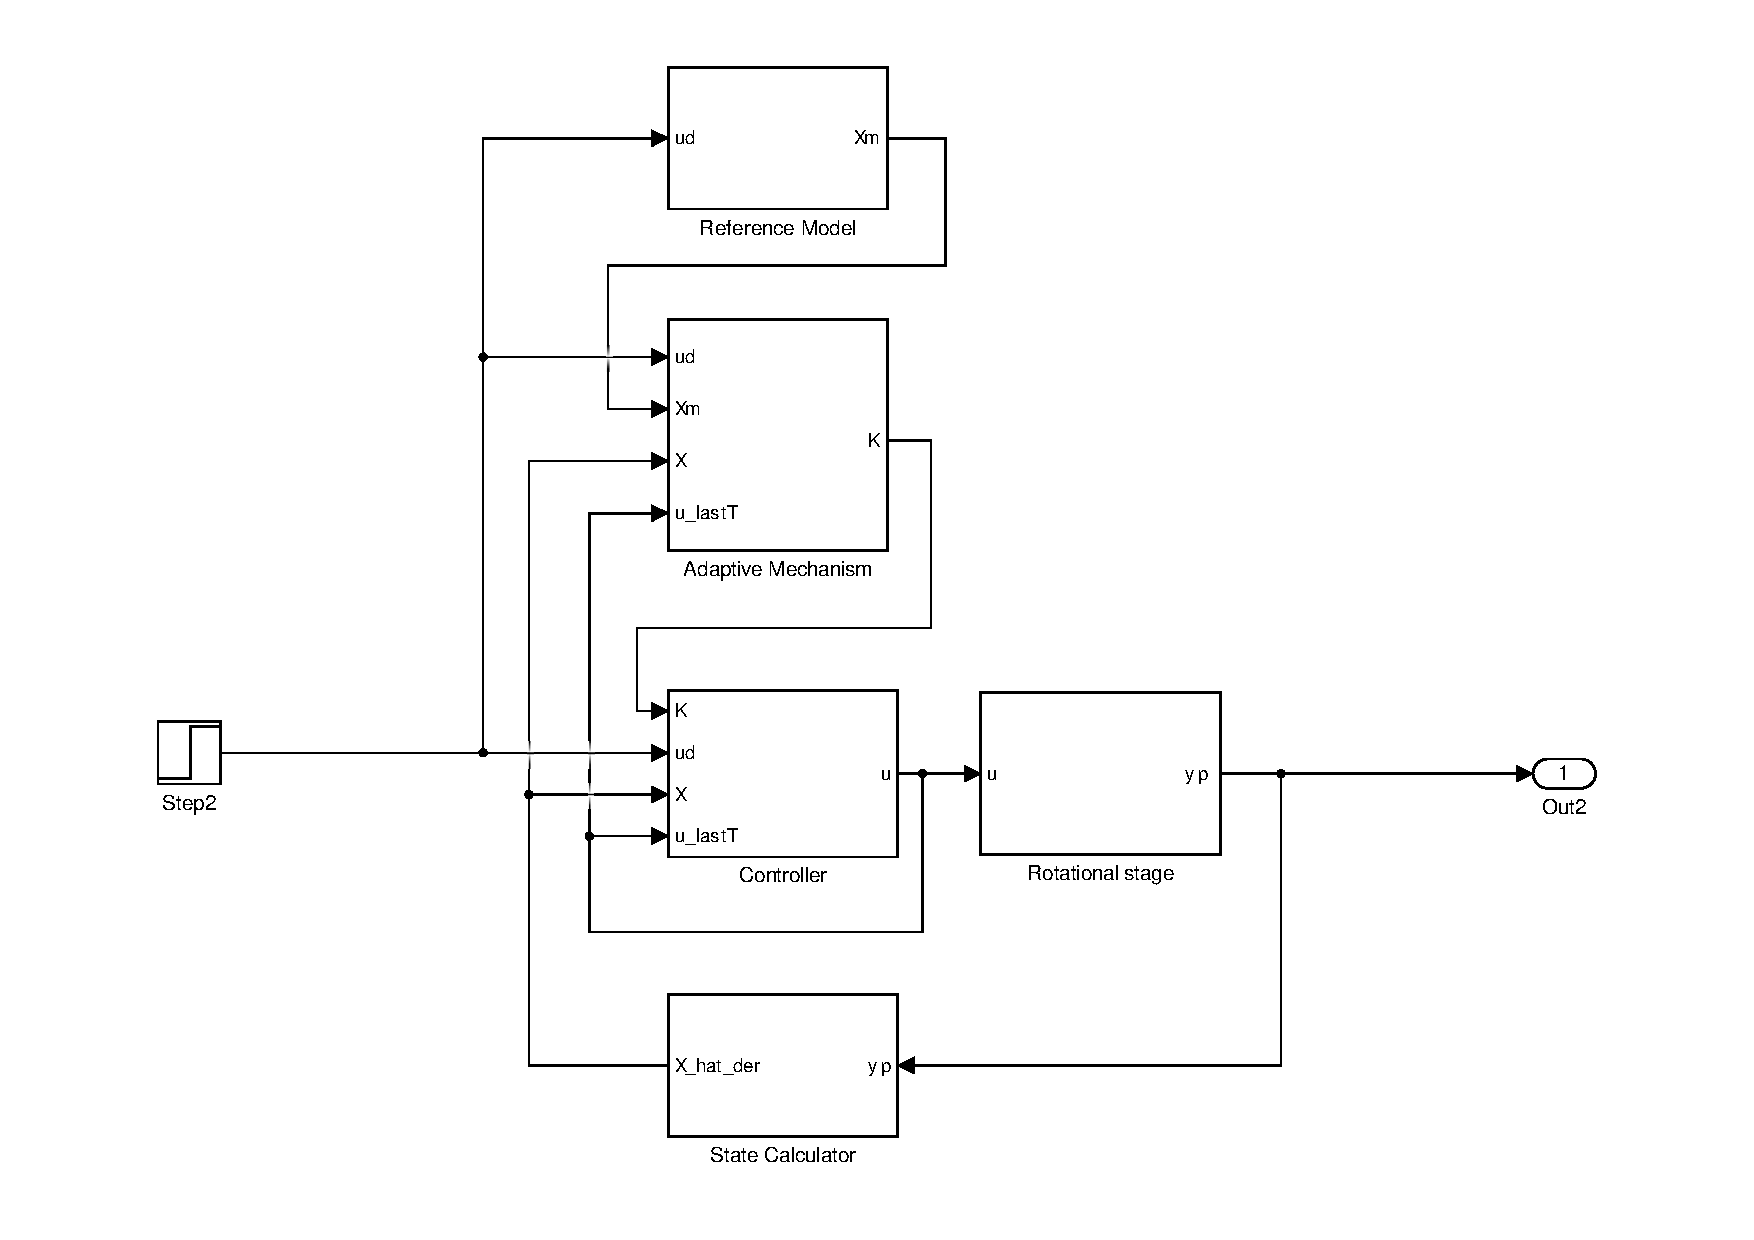
\includegraphics[width=0.7\textwidth, trim=4cm 0cm 3.8cm 0cm, clip=true]{fig/matlab/adaptive_scheme}
  \caption{\label{fig:adaptive}Block diagram of the adaptive controller}
\end{figure}

\section{Integral Resonance Control}
The integral resonace control (IRC) can be efficiently used to damp out the first resonant mode of the system, allowing for larger controller gains and a higher control bandwidth. The \abbrIRC scheme is illustrated in Figure~\ref{fig:irc} and consist of a constant artificial feed-through term $D_f<0$ and an integral controller $C=\frac{k}{s}$. The negative feed-forward term will, if sufficiently large and negative, introduce a pair of complex zeros below the first resonance frequency and ensure zero-pole cancellation for higher resonance modes as shown in \citep{Aphale:2007}. For stability, the phase response of the loop-gain $CG_d$ must be within $\pm180^{\circ}$ while the gain is greater than 0. The negative sign in $G_d$ subtracts a phase of $-180^{\circ}$. Using this knowledge, the phase margin can be easily increased by applying a simple negative integral controller to provide a 90 degrees phase lead. This results in a phase margin between  $\pm90^{\circ}$ which gives the system highly desired properties such as a $90^{\circ}$ phase margin and an infinte gain margin.

The negative gain $D_f$ is straight forward to manually select for introducing a complex pair of zeros below the first resonance. The integral gain $k$ can be choosen by using the root locus technique and select a gain that maximizes damping.

\begin{figure}[h]
  \centering %crop: left bottom right top
  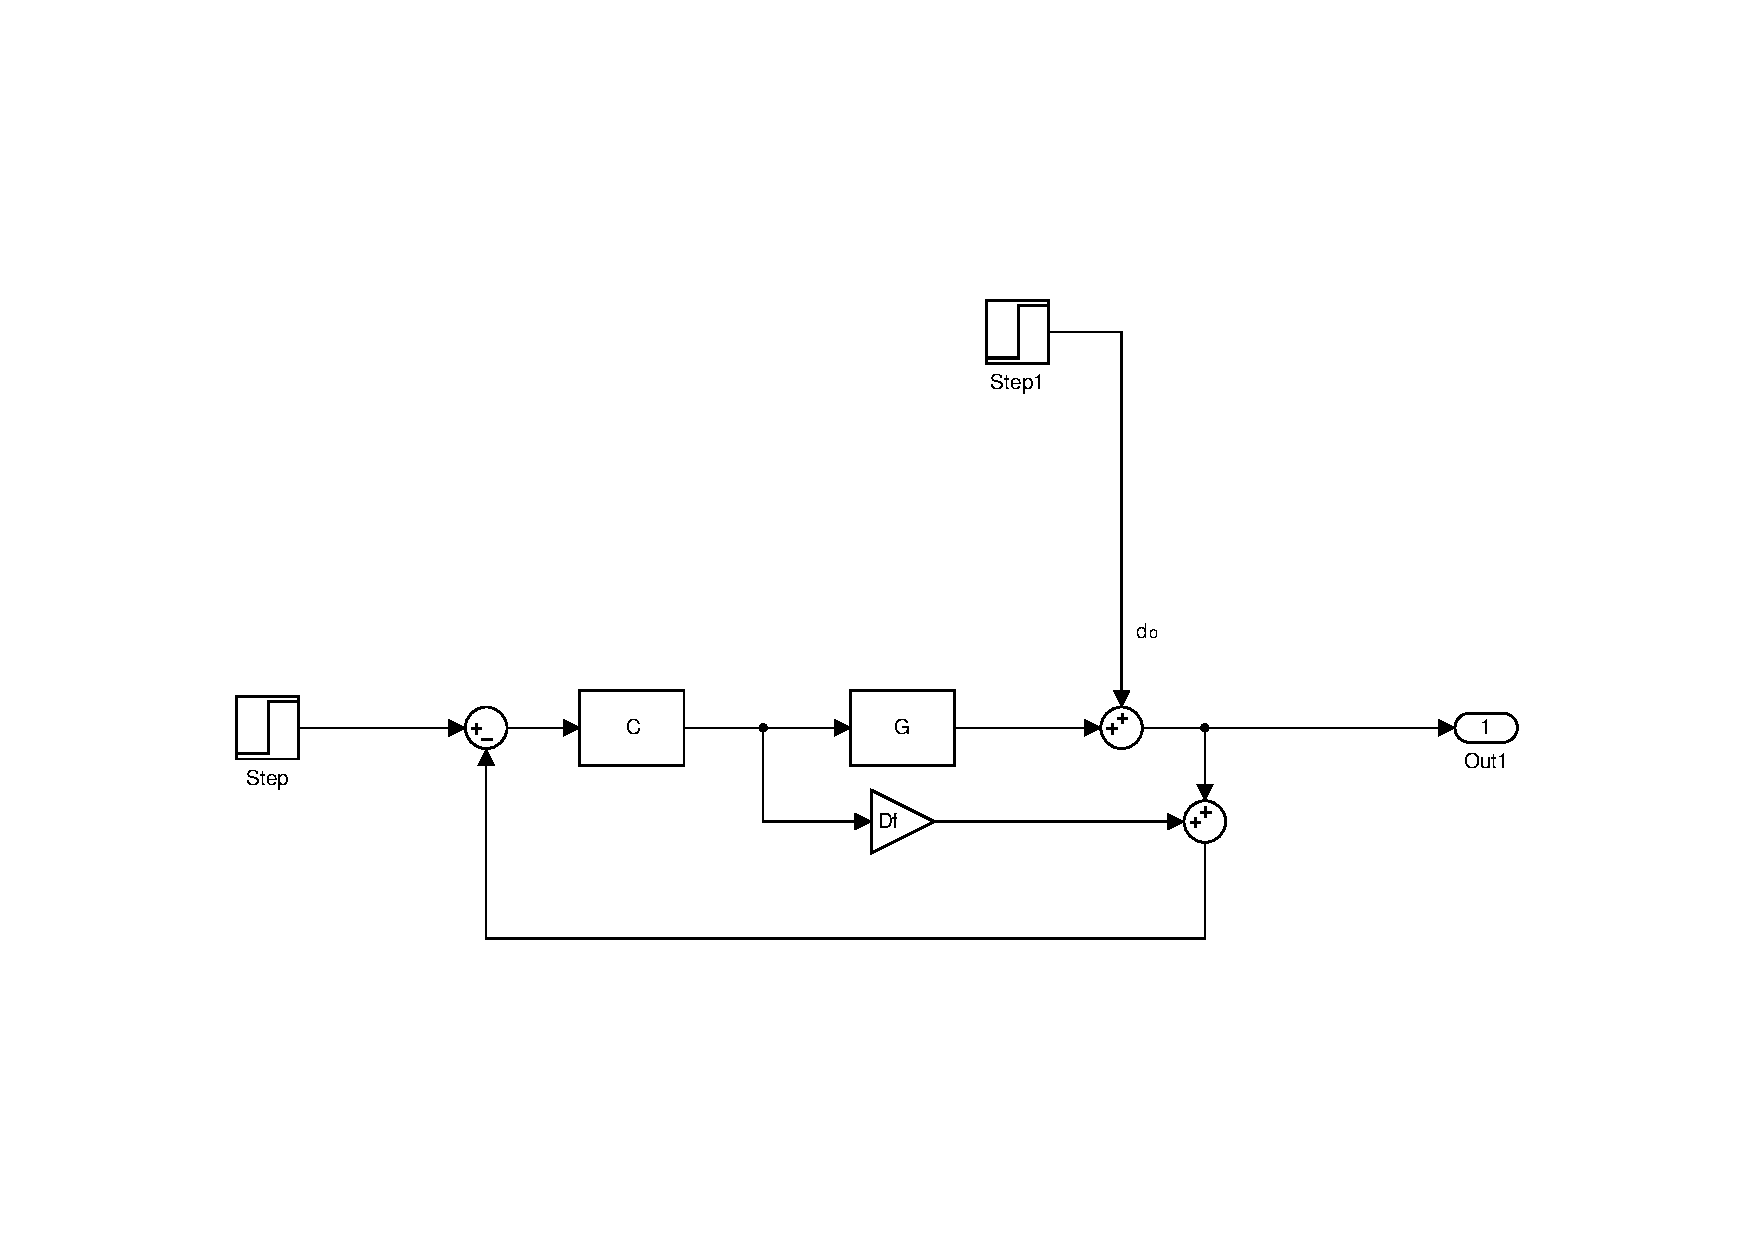
\includegraphics[width=1\textwidth, trim=5.5cm 3cm 5.1cm 9.5cm, clip=true]{fig/matlab/irc}
  \caption{\label{fig:irc}Block diagram of IRC damping loop}
\end{figure}

The IRC scheme in Figure~\ref{fig:irc} can be simplified, by combining $C$ and $D_f$ in the same block, the resulting scheme is shown in the inner loop in Figure~\ref{fig:irc_int}, where $C_2 = \frac{C}{1+CD_f}$. For tracking reference trajectories, the IRC can be enclosed in an outer loop, also seen in Figure~\ref{fig:irc_int}, utilizing a second controller $C_1$ to compensate for disturbances and model errors. For the outer controller $C_1$, a PI controller is sufficient but must include a negtive gain to compensate for the inversion that is caused by $D_f$ \citep{gu:2014}.

\begin{figure}[h]
  \centering %crop: left bottom right top
  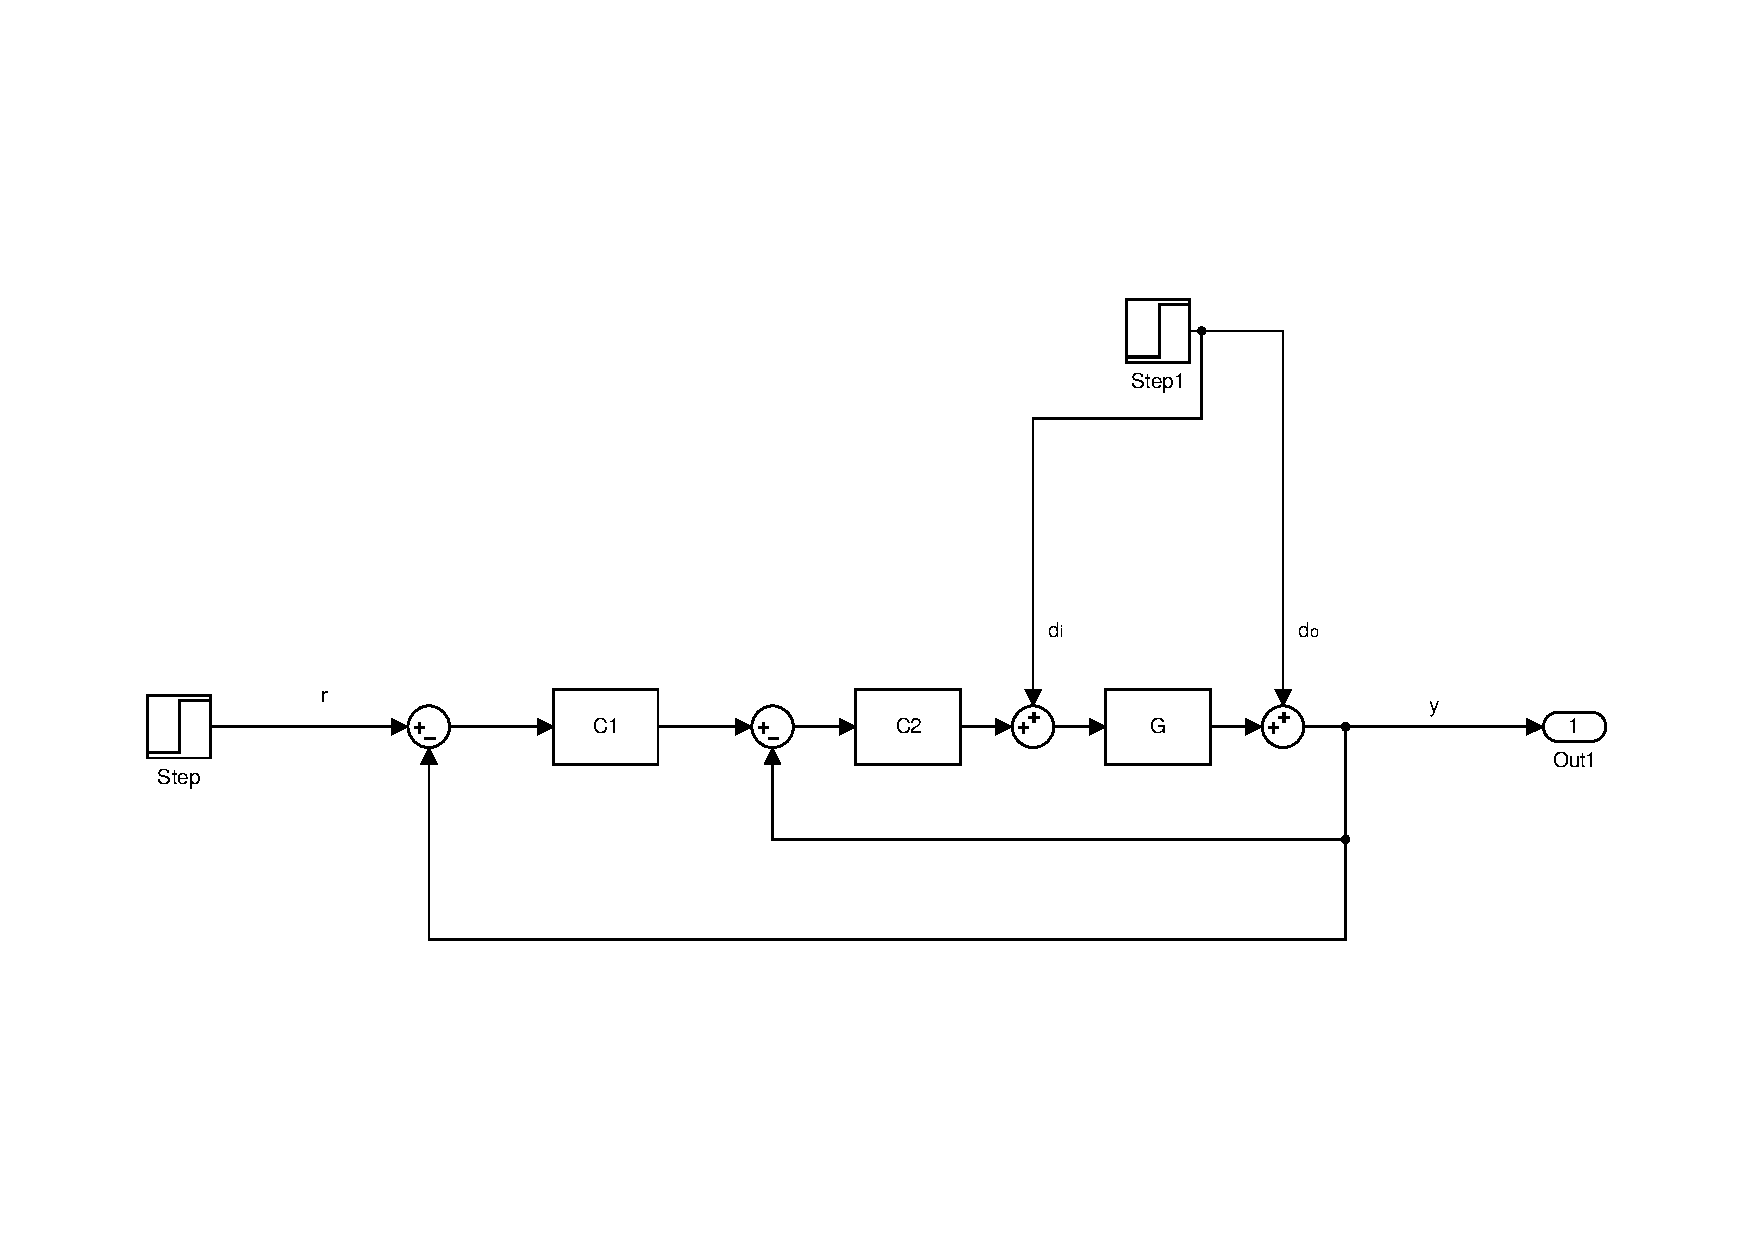
\includegraphics[width=1\textwidth, trim=4cm 5cm 3.6cm 9.5cm, clip=true]{fig/matlab/irc_int}
  \caption{\label{fig:irc_int}Block diagram of the tracking control system with IRC included}
\end{figure}

Proof for the zero-pole interlacement and the insertion of the complex conjugate zeros can be found in \citep{Aphale:2007}, but note that the proof is only given for causal systems with a relative degree of two i.e two more poles than zeros. To give the reader further information about the \abbrIRC and for a system with a relative degree of one, a brief example of a low order system is provided below.

Let G be represented as a transfer function with a relative degree of one, with 2 poles and 1 zero as written below,

\begin{equation}
  \label{eq:irc_sys}
  G = \frac{s + \alpha_0}{s^2 + \beta_1s + \beta_0}
\end{equation}

where  $\alpha_i > 0$ and  $\beta_i > 0$, i.e. a stable and minimum phase system.  Using $G_d = G + D_f$  ~\eqref{eq:irc_sys} and rearranging the terms gives

\begin{equation}
  \label{eq:irc_sys_d}
  \begin{split}
  G_d & = \frac{s + \alpha_0}{s^2 + \beta_1s + \beta_0} + D_f \\
      & = \frac{D_fs^2 + (1 + D_f\beta_1)s + \alpha_0 + D_f\beta_0}{s^2 + \beta_1s + \beta_0} \\
      & = \frac{D_f(s^2 + (\frac{1}{D_f} + \beta_1)s + \frac{\alpha_0}{D_f} + \beta_0)}{s^2 + \beta_1s + \beta_0}
  \end{split}
\end{equation}

which illustrates that the number of introduced zeros is equal to the relative degree of the transfer function and that the zeros ($s^z_i$) will have a negative real part if the following conditions are fullfilled.

\begin{equation}
  \label{eq:irc_cond}
  Re(s^z_i) < 0 \quad \text{if }
  \begin{cases}
    D_f < -\frac{1}{\beta_1}\\
    D_f < -\frac{\alpha_0}{\beta_0}\\
  \end{cases}
\end{equation}



%\begin{chapter-appendix}
%  \label{ap:lyaponov}

%\section{MRACPE}

%\end{chapter-appendix}
